\documentclass[11pt]{article}

\usepackage[margin=1in]{geometry}
\usepackage{amsmath,amssymb}
\usepackage{booktabs}
\usepackage{pgfplots}
\pgfplotsset{compat=1.17}
\usepackage[hidelinks]{hyperref}
\usepackage{parskip}

\title{From Ratios to Differential Equations:\\ A Geometric Model of a Strip with Three Subregions}
\author{}
\date{}

\begin{document}
\maketitle

\section{The model}

A rectangular strip has width $w$ and length $l$, so its area is
\[
  A = w\,l .
\]
The length is divided into three cell-boundary segments $r$, $o$, and $n$ with
\[
  l = r + o + n .
\]
Each subregion is a rectangle spanning the full width, with areas
\[
  a_r = w\,r, \qquad a_o = w\,o, \qquad a_n = w\,n,
\]
where the subscript names the region. These add back to the total:
$a_r + a_o + a_n = w(r+o+n) = w\,l = A$.

\section{Constant width: why ratios suffice}

If $w$ is held constant and only the length changes,
\[
  \Delta A = w\,\Delta l = w(\Delta r + \Delta o + \Delta n),
  \qquad \Delta a_r = w\,\Delta r, \ \text{etc.}
\]
Three facts make a differential equation unnecessary:

\begin{enumerate}
  \item \textbf{The derivative is constant.} $dA/dl = w$ and $d^2A/dl^2 = 0$. With no curvature, the difference quotient $\Delta A/\Delta l$ equals $dA/dl$ exactly for any size of change; taking a limit adds nothing.
  \item \textbf{Width cancels in every comparison.}
  \[
    \frac{a_r}{A} = \frac{w\,r}{w\,l} = \frac{r}{l},
    \qquad
    \frac{\Delta a_r}{\Delta A} = \frac{\Delta r}{\Delta l}.
  \]
  The problem reduces to one-dimensional proportions along the length.
  \item \textbf{There is no feedback.} A differential equation is needed when a rate depends on the current state (e.g.\ $dA/dt = kA$). Here the area gained per unit length does not depend on the current length or how it is divided.
\end{enumerate}

\section{Width and length both change}

\subsection{The product rule}

The rate of change of a product is not the product of the rates. If $A = w\,l$ with both varying in time,
\[
  \frac{dA}{dt} = w\,\frac{dl}{dt} + l\,\frac{dw}{dt}.
\]

\subsection{Where the ``product of changes'' lives}

For a finite change,
\[
  \Delta A = (w+\Delta w)(l+\Delta l) - w\,l
  = w\,\Delta l + l\,\Delta w + \Delta w\,\Delta l .
\]
The term $\Delta w\,\Delta l$ is the small corner rectangle that appears when the strip grows in both directions at once. It is second-order:
\[
  \frac{\Delta w\,\Delta l}{\Delta t} = \frac{\Delta w}{\Delta t}\,\Delta l \;\longrightarrow\; \frac{dw}{dt}\cdot 0 = 0,
\]
so it vanishes from the derivative but is real for any finite step. This is why simple ratios stop being exact once both dimensions change.

\subsection{Subareas and shares}

Each subarea obeys the same rule:
\[
  \frac{da_r}{dt} = w\,\frac{dr}{dt} + r\,\frac{dw}{dt}.
\]
The term $r\,dw/dt$ means widening adds area to every region in proportion to its current length, even a region whose boundaries are not moving. Yet the shares are still
\[
  \frac{a_r}{A} = \frac{r}{l}.
\]
These statements do not conflict: the first concerns \emph{absolute} gains, the second \emph{proportions}.

\paragraph{Example.} Take $r=1$, $o=3$, $n=6$ ($l=10$) and widen from $w=2$ to $w=3$ with no boundaries moving.

\begin{center}
\begin{tabular}{lccccc}
\toprule
Region & Area ($w=2$) & Area ($w=3$) & Gain & Growth & Share \\
\midrule
$r$ & 2  & 3  & $+1$  & 50\% & 10\% $\to$ 10\% \\
$o$ & 6  & 9  & $+3$  & 50\% & 30\% $\to$ 30\% \\
$n$ & 12 & 18 & $+6$  & 50\% & 60\% $\to$ 60\% \\
\midrule
Total & 20 & 30 & $+10$ & 50\% & \\
\bottomrule
\end{tabular}
\end{center}

\subsection{Relative rates add}

Dividing the product rule by $A = w\,l$:
\[
  \frac{1}{A}\frac{dA}{dt} = \frac{1}{w}\frac{dw}{dt} + \frac{1}{l}\frac{dl}{dt},
  \qquad\text{i.e.}\qquad
  \frac{d\ln A}{dt} = \frac{d\ln w}{dt} + \frac{d\ln l}{dt}.
\]
Per region,
\[
  \frac{1}{a_r}\frac{da_r}{dt} = \frac{1}{w}\frac{dw}{dt} + \frac{1}{r}\frac{dr}{dt}.
\]
The width term is identical for every region, so width alone can never change the shares; only unequal length terms can.

\section{The picture-resize analogy}

Think of the strip as an image of three vertical stripes, lengths $r$, $o$, $n$ left to right, each spanning the full height $w$.

\begin{itemize}
  \item \textbf{Drag the top or bottom edge} (change $w$ only): every stripe gets taller by the same factor; boundaries do not move; shares are unchanged.
  \item \textbf{Drag a side edge} (resize length): the editor stretches the image evenly, so each boundary moves in proportion,
  \[
    \frac{dr}{dt} = \frac{r}{l}\,\frac{dl}{dt}, \quad\text{and likewise for } o, n,
  \]
  and the shares are again unchanged.
  \item \textbf{Drag a corner} (change both): each stripe's area is multiplied by (width factor)$\times$(length factor). Scaling both by $1.5$ multiplies every area by $2.25$; the split stays $10/30/60$.
  \item \textbf{Crop or change canvas size}: boundaries move unevenly (e.g.\ only $n$ extends), and shares \emph{do} change. This is the general case of the model.
\end{itemize}

\section{Tying the boundaries to the width}

\subsection{The sum condition is automatic}

Since $l = r + o + n$ at all times, differentiating gives
\[
  \frac{dr}{dt} + \frac{do}{dt} + \frac{dn}{dt} = \frac{dl}{dt}
\]
for free. The real content of the model is how each boundary depends on $dw/dt$.

\subsection{Time drops out}

If $dr/dt = f_r\cdot dw/dt$, dividing by $dw/dt$ gives
\[
  \frac{dr}{dw} = f_r .
\]
Plot width against a boundary length: as the picture's edge is dragged, the stripe's corner traces a path in the $(w,r)$ plane, and $dr/dw$ is the slope of that path. Time sets only how fast the edge is dragged, not the path. The full model is
\[
  \frac{dr}{dw} = f_r,\quad \frac{do}{dw} = f_o,\quad \frac{dn}{dw} = f_n,\qquad A = w(r+o+n).
\]

\subsection{Three cases}

\paragraph{Case 1: fixed ratio of changes.} $dr/dw = c_r$ (constant). Then $r = r_0 + c_r(w - w_0)$, a straight line, and $\Delta r/\Delta w = c_r$ exactly. The rule does not depend on the state; it is technically a differential equation, but a trivial one. All solutions are parallel lines.

\paragraph{Case 2: rate set by the stripe's own size.}
\
  \frac{dr}{dw} = \frac{r}{w}.
\]
Separating variables, $dr/r = dw/w$, so $\ln r = \ln w + C$ and
\[
  r = \frac{r_0}{w_0}\,w .
\]
The rule depends on the current state, which makes this a differential equation with real content. Its solutions nonetheless have constant slope $dr/dw = r_0/w_0$: they are rays through the origin, with the slope fixed by the starting point. This is the locked-aspect-ratio resize; shares never change.

\begin{center}
\begin{tabular}{lcc}
\toprule
Stripe & Length at $w=2$ & Slope $dr/dw = \text{length}/w$ \\
\midrule
$r$ & 1 & 0.5 \\
$o$ & 3 & 1.5 \\
$n$ & 6 & 3 \\
\bottomrule
\end{tabular}
\end{center}

Case 1 needs the three slopes supplied separately; Case 2 computes them from the state. Both give straight paths: Case 1 a family of parallel lines, Case 2 a fan of rays.

\paragraph{Case 3: stripes respond differently.}
\[
  \frac{dr}{dw} = k_r\,\frac{r}{w}
  \quad\Longrightarrow\quad
  r = r_0\left(\frac{w}{w_0}\right)^{k_r},
\]
with a separate constant for each stripe. For $k \neq 1$ the paths curve, and because stripes follow different powers of $w$, widening redistributes the area.

\subsection{The response constant \texorpdfstring{$k$}{k}}

Rearranging the Case~3 rule,
\[
  k_r = \frac{dr/r}{dw/w}
  = \frac{\text{percentage change in } r}{\text{percentage change in } w}.
\]
If the width grows by 1\%, stripe $r$'s length grows by about $k_r$ percent. For example, with $w=2$, $r=1$, $k_r=2$, widening to $w=2.02$ gives $r \approx 1.02$.

\begin{center}
\begin{tabular}{lll}
\toprule
$k$ & Effect as the picture widens & In the picture \\
\midrule
$k=0$ & length unchanged & stripe only gets taller \\
$0<k<1$ & length grows by a smaller \% than width & relatively taller and narrower \\
$k=1$ & same \% as width & shape kept (locked-aspect resize) \\
$k>1$ & larger \% than width & stretches out faster than it grows taller \\
$k<0$ & length shrinks & stripe squeezed \\
\bottomrule
\end{tabular}
\end{center}

Doubling the width multiplies a stripe's length by $2^k$. The values below are illustrative choices; in a real model, $k$ would be assumed from the underlying biology or physics, or measured as the slope of $\ln r$ against $\ln w$.

\subsection{Worked example and figure}

With $w_0 = 2$, $r_0=1$, $o_0=3$, $n_0=6$ and $k_r=2$, $k_o=1$, $k_n=0.5$:
\[
  r = \left(\tfrac{w}{2}\right)^2,\qquad
  o = 1.5\,w,\qquad
  n = 6\sqrt{\tfrac{w}{2}} .
\]
At $w=4$: $r = 4$, $o = 6$, $n \approx 8.49$, so the shares move from $10/30/60$ to about $22/32/46$.

\begin{center}
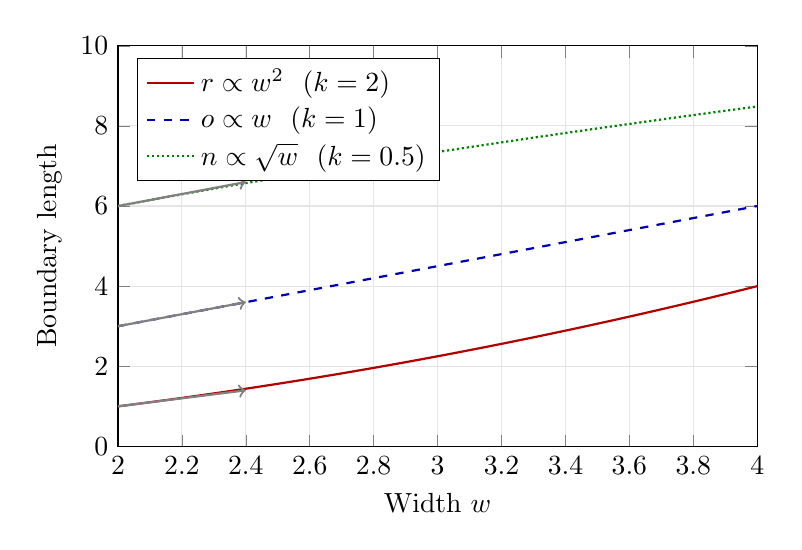
\begin{tikzpicture}
\begin{axis}[
  width=0.8\textwidth, height=0.55\textwidth,
  xlabel={Width $w$}, ylabel={Boundary length},
  xmin=2, xmax=4, ymin=0, ymax=10,
  legend pos=north west, legend cell align=left,
  grid=major, grid style={gray!20},
]
\addplot[domain=2:4, samples=60, thick, red!70!black]                 {(x/2)^2};
\addlegendentry{$r \propto w^2$ \ ($k=2$)}
\addplot[domain=2:4, samples=2,  thick, dashed, blue!70!black]        {1.5*x};
\addlegendentry{$o \propto w$ \ ($k=1$)}
\addplot[domain=2:4, samples=60, thick, densely dotted, green!50!black] {6*sqrt(x/2)};
\addlegendentry{$n \propto \sqrt{w}$ \ ($k=0.5$)}
% tangent directions at w = 2 (slopes 1, 1.5, 1.5)
\draw[->, gray, thick] (axis cs:2,1) -- (axis cs:2.4,1.4);
\draw[->, gray, thick] (axis cs:2,3) -- (axis cs:2.4,3.6);
\draw[->, gray, thick] (axis cs:2,6) -- (axis cs:2.4,6.6);
\end{axis}
\end{tikzpicture}
\end{center}

The gray arrows at $w=2$ are the differential equation itself: at each point the rule gives only the direction of the next small step. Taking a tiny straight step, recomputing the rule, and repeating stitches those straight pieces into the curve, the reverse of zooming in until a curve looks straight.

\section{Where the model goes next}

So far each stripe's rule depends only on its own length and the width. A more realistic model couples the regions, for example letting the boundary between $r$ and $o$ move according to the difference in their sizes:
\[
  \frac{dr}{dw} = f_r(r,o,n,w),\quad
  \frac{do}{dw} = f_o(r,o,n,w),\quad
  \frac{dn}{dw} = f_n(r,o,n,w).
\]
The stripes can no longer be solved separately; the direction of motion lives in the full $(r,o,n)$ space. At that point a differential-equation description is unavoidable, since no simple ratio or power law captures the interaction.

\end{document}
